%%%%%%%%%%%%%%%%%%%%%%%%%%%%%%%%%%%%%%%%%%%%%%%%%%%%%%%%%%%%%%%%%%%%%%%%%%%%%%%%
%                               ANALYSE SIMUS CHES                             %
%%%%%%%%%%%%%%%%%%%%%%%%%%%%%%%%%%%%%%%%%%%%%%%%%%%%%%%%%%%%%%%%%%%%%%%%%%%%%%%%
\begin{figure}
    \centering
    \begin{subfigure}{0.49\textwidth}
        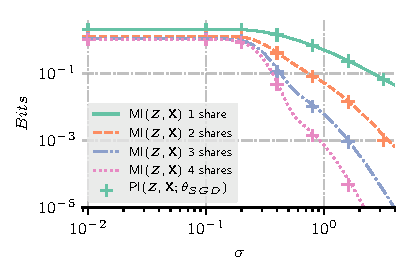
\includegraphics{Figures/simus/MI_bool_exp1_05}
        \caption{Experiment 1}
        \label{fig:exp_MI_1}
    \end{subfigure}
    \begin{subfigure}{0.49\textwidth}
        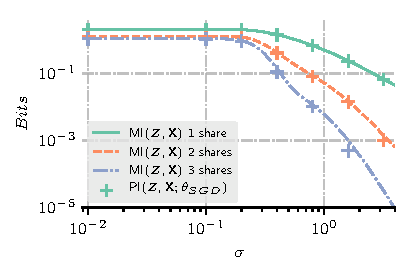
\includegraphics{Figures/simus/MI_bool_exp2_05}
        \caption{Experiment 2}
        \label{fig:exp_MI_2}
    \end{subfigure}
    \begin{subfigure}{0.49\textwidth}
        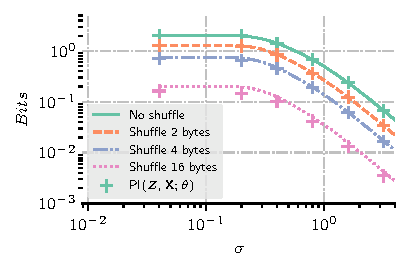
\includegraphics{Figures/simus/shuffle_simus}
        \caption{Experiment 3}
        \label{fig:exp_MI_3}
    \end{subfigure}
	\caption{Information perceived by the \gls{mlp}.}
	\label{fig:exp_MI}
\end{figure}


In this section we analyze the results obtained by running Experiments \(1\) (\autoref{fig:exp_MI_1}), \(2\) (\autoref{fig:exp_MI_2}) and \(3\) (\autoref{fig:exp_MI_3}).
On each figure, the lines correspond to the estimated \gls{mi} and the crosses correspond to the information perceived by the trained \gls{mlp}, as computed from the \gls{nll} loss with \autoref{eq:PI_eq_gen_loss}.
Based on these results, several observations can be done.

First, on each result the crosses are always below the lines, which is in line with the results given in the literature: the estimated \gls{pi} is a lower bound of the \gls{mi}. 
But more interestingly, the crosses are always close to the line no matter the \gls{mi} magnitude.
In the case of Experiment 1, we argued that the error was composed of the approximation and optimization errors, so their sum is negligible.
Since we recalled in \autoref{sec:div_term} that those terms are both negative, we conclude that even for a simple \gls{mlp} with one layer and \(1,000\) neurons, both errors can be ignored. 
This is of particular interest concerning the approximation error, as it always decreases with the number of layers and the number of neurons inside each layer of the \gls{mlp}. 
Therefore, in the case of a Hamming weight leakage model with additive Gaussian noise, any \textit{more sophisticated} \gls{mlp} (\ie{} with more layers or more neurons by layer) will also have a negligible approximation error.

Secondly, the \gls{pi} plotted in \autoref{fig:exp_MI_2} shows that the presence of uninformative components in Experiment 2 does not annihilate the capacity of the \gls{mlp} to optimally extract information about the target variable, provided that these components are not shuffled with informative ones.
This shows that the optimization error, which was thought to be increased compared to Experiment 1, remains stable.

Finally, the preceding observations hold regardless the considered counter-measure, namely secret-sharing (\autoref{fig:exp_MI_1} and \autoref{fig:exp_MI_2}) or shuffling (\autoref{fig:exp_MI_3}).
This can be interpreted as the fact that the \gls{mlp} trained through the \gls{nll} loss minimization is able to give a model optimally extracting the remaining informative leakage, while being ``agnostic'' concerning the presence or not of such counter-measures.
Nevertheless, since both counter-measures have been shown to decrease the \gls{mi} -- exponentially with the level of noise for secret-sharing as explained in \autoref{sec:masking} or linearly for shuffling as explained in \autoref{sec:hiding} -- they remain sound against Deep Learning.

At this stage, we have argued thanks to our simulations that the approximation error is negligible, no matter the considered counter-measure, nor the architecture of a \gls{mlp}, while the optimization error is likely to remain negligible as well.
Therefore, our \gls{mi} estimation obtained by \gls{pi} maximization seems accurate. 
This provides an empirical validation of \autoref{prop:cor_sup_PI}.
As another consequence, we are fairly confident that in the case of such simple leakage models, which often happen on real use cases, replacing an optimal architecture by another should not degrade too much the \gls{mi} estimation.%
\footnote{However, one cannot get such a conclusion if one considers another leakage model.}
These observations must be challenged by tests on experimental traces, where one cannot have an exhaustive dataset. 
This will naturally lead to discussions regarding the estimation error which has not been investigated here.